\documentclass{article}

\usepackage[francais]{babel}
\usepackage[utf8]{inputenc}
\usepackage[T1]{fontenc}
\usepackage{graphicx}

\title{LOG6302 : Quiz 1}
\author{Troclet Philippe \textit{1815208}}
\date{\today}



\begin{document}
	\maketitle
	
\section{Application des techniques de réingénérie}
	Une première application serait le calcul de métrique à partir d'une base de code. Une second application serait la génération de diagramme UML. Ces applications nécessitent de construire l'arbre de parsage puis de le parcourir. On remarque qu'on pourrait également réaliser ces applications via des traductions dirigées par la syntaxe.
\section{\'Etude d'une grammaire}
	\subsection*{Question a}
	 Les non-terminaux de cette grammaire sont \textit{bexpr},\textit{bterm} et \textit{bfactor}. Les terminaux quant à eux sont 
	 \textbf{or}, \textbf{and}, \textbf{not},\textbf{(} et \textbf{(}. Enfin le symbole \textit{Start} est \textit{bexpr}. En effet,
	 les non-terminaux sont l'ensemble des symboles que l'on peut retrouver en partie gauche d'une règle. Les terminaux sont alors l'ensemble des symboles qui ne sont pas des non-terminaux. Enfin, les règles de production sont les suivantes:
	 \begin{enumerate}
		\item $\textit{bexpr} \rightarrow \textit{bexpr}\  \textbf{or}\ \textit{bexpr}$
		\item $\textit{bexpr} \rightarrow \textit{bterm}$
		\item $\textit{bterm} \rightarrow \textit{bterm}\  \textbf{and}\ \textit{bterm}$
		\item $\textit{bterm} \rightarrow \textit{bfactor}$
		\item $\textit{bfactor} \rightarrow \textbf{not}\  \textit{bfactor}$
		\item $\textit{bfactor} \rightarrow \textbf{(} \textit{bexpr} \textbf{)}$
		\item $\textit{bfactor} \rightarrow \textbf{true}$
		\item $\textit{bfactor} \rightarrow \textbf{false}$
	 \end{enumerate}
 
 \subsection*{Question b}
 	D'après la question précédente, il y a 8 règles de production.
 	
 \subsection*{Question c}
 	Le \textit{xor} et le ~ ne font pas partie de la grammaire aussi les deux derniers ne peuvent appartenir au langage. En conséquence, seul \textbf{not true and false} fait partie du langage.
 	
 	\subsection*{Question d}
 %	\subsubsection*{d.1}
 %	\subsubsection*{d.2}
 %Les deux dérivations donnent le même résultats, est-ce %normal?
 \begin{figure}[h]
 	\centering
 	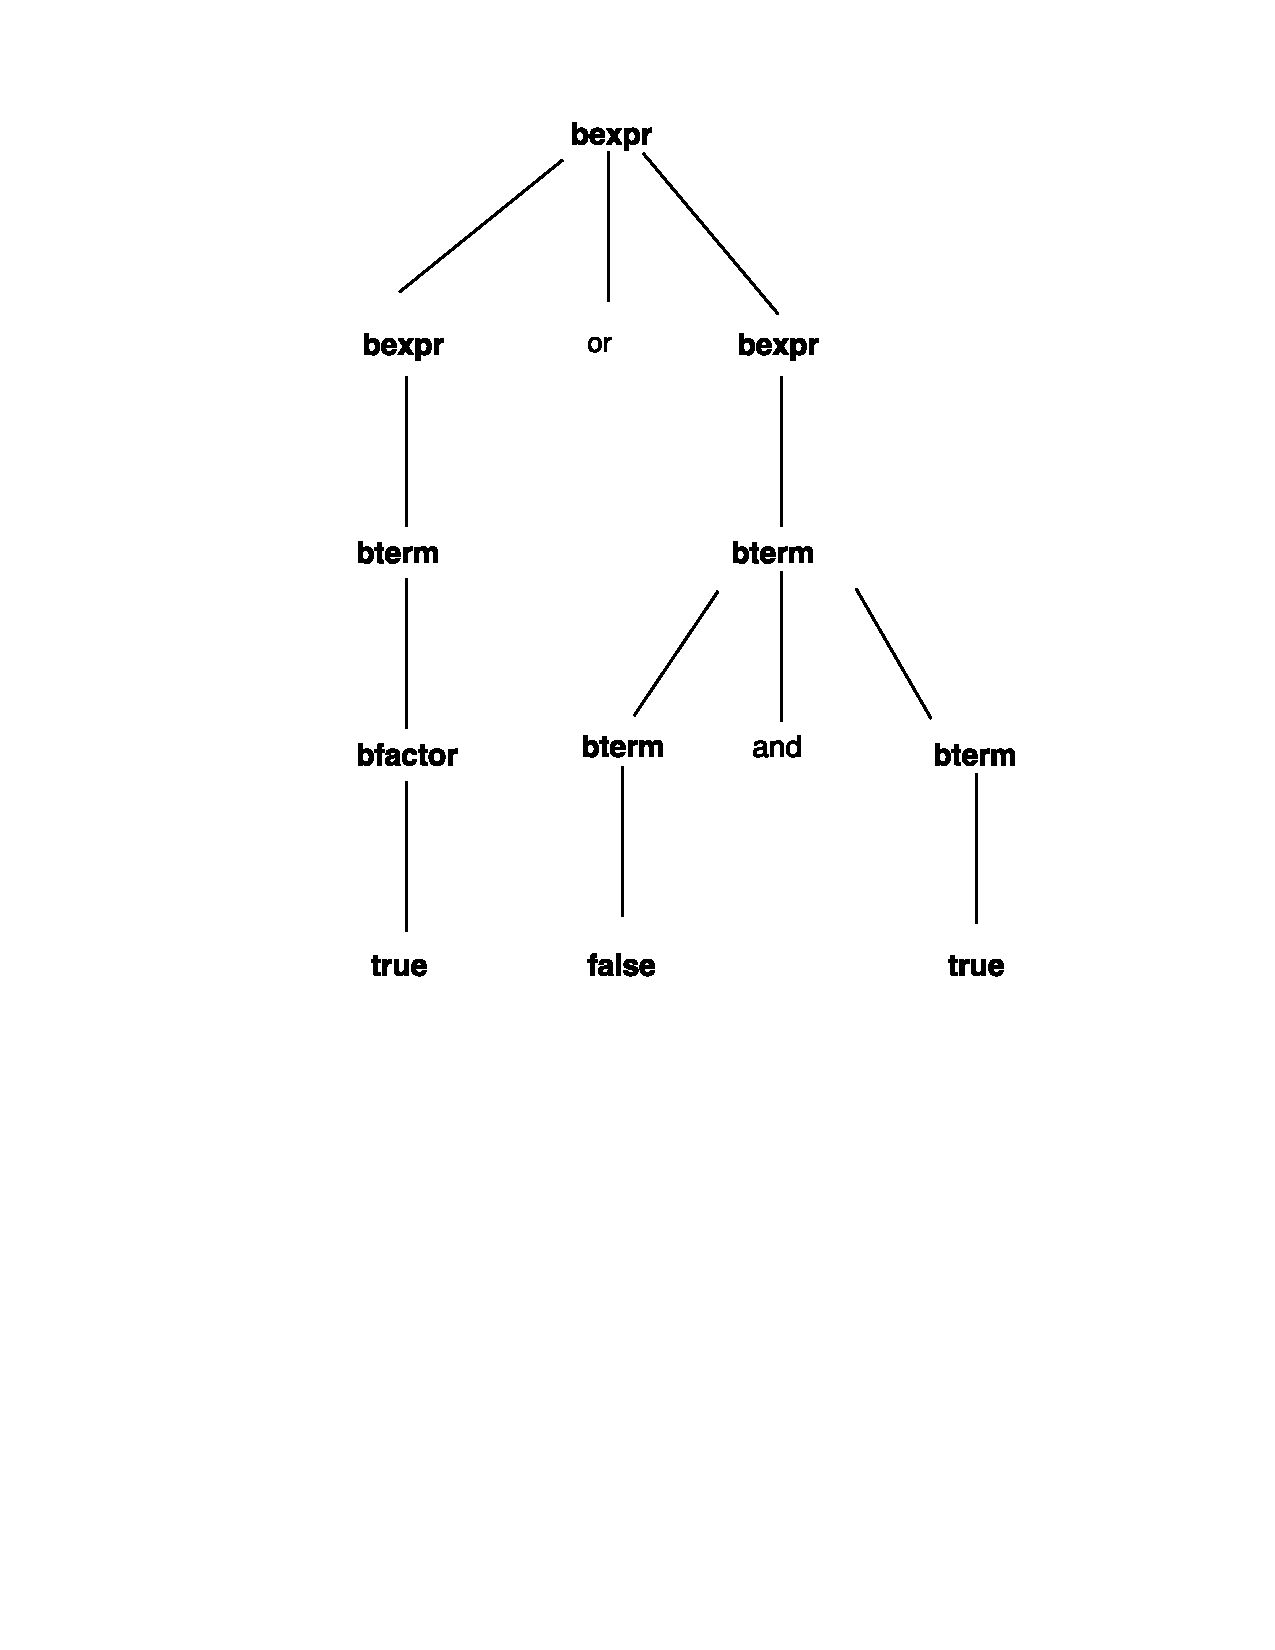
\includegraphics[width=0.7\linewidth]{Images/AST}
 	\caption[AST]{Arbre de syntaxe pour \textbf{true or false and true}}
 	\label{fig:ast}
 \end{figure}
 Les deux arbres de parsage sont identiques, on peut voir l'arbre correspondant sur la figure \ref{fig:ast}.
 
 \subsection*{Question e}
 La grammaire considérée ici est ambiguë, on peut pour cela étudier la chaîne \textbf{true or false or true}. En effet, selon qu'on suive une dérivation à gauche ou à droite, on obtient un arbre de parsage différent.
\section{Modification d'une grammaire}
Afin d'introduire un \textbf{xor}, nous proposons la grammaire suivante:
\begin{enumerate}
	\item $\textit{bexpr} \rightarrow \textit{bexpr}\  \textbf{or}\ \textit{bexpr}$
	\item $\textit{bexpr} \rightarrow \textit{exprxor}$
	\item $\textit{exprxor} \rightarrow \textit{exprxor}\  \textbf{xor}\ \textit{exprxor}$
	\item $\textit{exprxor} \rightarrow \textit{bterm}$
	\item $\textit{bterm} \rightarrow \textit{bterm}\  \textbf{and}\ \textit{bterm}$
	\item $\textit{bterm} \rightarrow \textit{bfactor}$
	\item $\textit{bfactor} \rightarrow \textbf{not}\  \textit{bfactor}$
	\item $\textit{bfactor} \rightarrow \textbf{(} \textit{bexpr} \textbf{)}$
	\item $\textit{bfactor} \rightarrow \textbf{true}$
	\item $\textit{bfactor} \rightarrow \textbf{false}$
\end{enumerate}
	
\section{Création d'une grammaire}
Afin de pouvoir reconnaître les numéros de téléphone canadiens, nous proposons la grammaire suivante:
\begin{itemize}
	\item $\textit{S} \rightarrow (+1) \textit{num} | \textit{num}$
	\item $\textit{num} \rightarrow \textit{C}\textit{C}\textit{C}\  \textit{C}\textit{C}\textit{C}\  \textit{C}\textit{C}\textit{C}\textit{C}$
	\item $\textit{C} \rightarrow 0 | 1| 2| 3 | 4 | 5 | 6 | 7 | 8 | 9 $
\end{itemize}
\end{document}
